\documentclass{article}

\usepackage{pdfpages}
\usepackage{graphicx}
\usepackage[export]{adjustbox}
\usepackage{tabu}
\usepackage{xcolor,colortbl}

\begin{document}

\vspace*{3ex}
\begin{flushright}
{\large 1 April 2015}
\end{flushright}

\begin{flushleft}
{\large Jakub Ciecierski\\

}
\end{flushleft}

\hskip3cm

\begin{center}

\Large {\bf
	Cellular automaton
}

\Large {\bf 
	Technical documentation 
}

\vskip2ex

\vspace{60pt}

\includegraphics[width=80mm]{images/mini.png} \\
\end{center}

\vskip20ex

\newpage

	\tableofcontents
	
\newpage


\section{Document metric}

\begin{table}[h]
\hspace*{-3.1cm}
\large
\begin{tabular}{|
>{\columncolor[HTML]{C0C0C0}}l |l|l|l|l|l|}
\hline
\multicolumn{6}{|l|}{\cellcolor[HTML]{C0C0C0}Document metric}                                                                                                                                         \\ \hline
Project:       & Cellular Automaton                                                       & \cellcolor[HTML]{C0C0C0}Company: & \multicolumn{3}{l|}{WUT}                                               \\ \hline
Name:          & \multicolumn{5}{l|}{Technical Documentation}                                                                                                                                       \\ \hline
Topics:        & \multicolumn{5}{l|}{Technical Documentation}                                                                                                                                       \\ \hline
Author:        & \multicolumn{5}{l|}{Jakub Ciecierski}                                                                                                                                                \\ \hline
File:          & \multicolumn{5}{l|}{technical.pdf}                                                                                                                                      \\ \hline
Version no:    & 0.1                                                                      & \cellcolor[HTML]{C0C0C0}Status:  & Under development & \cellcolor[HTML]{C0C0C0}Opening date: & 2015-03-03 \\ \hline
Summary:       & \multicolumn{5}{l|}{Technical documentation for cellular automaton}                                                                                                           \\ \hline
Authorized by: & \begin{tabular}[c]{@{}l@{}}Władysław Homenda\\ Lucjan Stapp\end{tabular} & \multicolumn{3}{l|}{\cellcolor[HTML]{C0C0C0}Last modification date:}                         & 2015-04-01 \\ \hline
\end{tabular}
\end{table}



\section{History of changes}

	\begin{table}[h]
		\hspace*{-2.1cm}
		\large
		\begin{tabular}{|l|l|l|l|}
		\hline
		\multicolumn{4}{|l|}{\cellcolor[HTML]{C0C0C0}History of Changes} \\ \hline
		Version         & Date         & Who        & Description        \\ \hline
		0.1         & 2015-04-01         & Jakub Ciecierski        & Definition of the main purpose of the document       \\ \hline
		\end{tabular}
	\end{table}

\newpage




\section{Technology}

The technology of my choice is C\# programming language under .NET framework.
It is known to be a robust tool which allows for relatively easy creation
of complex applications.





\section{Algorithms}

\subsection{Rule}

Algorithm for creating {\bf Rules} has been prepared thoroughly to yield a robust and flexible
way to implement transition of generation.

\subsubsection{Definitions}

We define {\bf Rule} as a set of {\bf Transitions} each having {\bf Transition Function} 
which computes if {\bf Cell} 
belonging in input {\bf Neighborhood} should transition to {\bf New State}.

{\bf Rule} is equipped with a {\bf default Transition} which is used for transitions
for neighborhoods for which no transition was defined - it can simply be a transition which
does not change a state

\subsubsection{Algorithms}
% Begin algorithms
\begin{itemize}
\item {\bf Creating Rule}
	\begin{enumerate}
		\item Create {\bf Rule} for given {\bf Neighborhood Type}
		\item Create a {\bf Transition} we want to add to Rule set:
			\begin{enumerate}
				\item Define a custom {\bf Transition Function} which takes a 
				neighborhood and returns a boolean value			
				\item Define {\bf New State} to which a Cell in valid neighborhood should transition.
				\item Add {\bf Transition} to {\bf Rule}.
			\end{enumerate}
		\item Repeat Point 2. to add more {\bf Transitions}
	\end{enumerate}

\item {\bf Apply Rule}\\
	{\bf Input:} {\bf Neighborhood}. 
	{\bf Output:} {\bf New state}
	\begin{enumerate}
		\item Look for proper Transition which will successfully apply to input 
		Neighborhood.
		\item If no Transition Function was defined for this neighborhood, apply Default Transition
	\end{enumerate}

% End algorithms
\end{itemize}

\subsubsection{Examples}

% Being Examples
\begin{itemize}

\item Example 1 {\bf Creating Rule}
\begin{enumerate}
	\item User selects {\bf Rule} for 4-point neighborhood - {\bf Rule} is created.
	
	\item User wants to add a transition for specific layout of neighbors (in specific states) -
	{\bf Transition} is created.
	
	\begin{enumerate}

		\item A 4-point neighborhood NB\_U is created based on the user's choice:
		
		\begin{itemize}
			\item Local Cell State: '0'
			\item Upper and Bottom neighbor State: '1'
			\item Left and Right neighbors State: '0'
 		\end{itemize}
 		
		{\bf Transition Function} is defined so that it accepts transition if input neighborhood 
		NB\_I is exactly equal to NB\_U
		
		\item {\bf New State}: '1' is defined from user's choice
		
		\item {\bf Transition} is added to {\bf Rule} set
			
	\end{enumerate}	
\end{enumerate}


\item Example 2 {\bf Creating Rule}
\begin{enumerate}
	\item User selects {\bf Rule} for 24-point neighborhood - {\bf Rule} is created.
	\item User wants to add a transition stating that 5 neighbors should be in state '1',
	4 neighbors should be in state '0' and Local State should be in state '0' - 
	{\bf Transition} is created.
	\begin{enumerate}

		\item A Transition Function is defined as follow: \\
		If input neighborhood NB\_I has 5 cell in state '1' AND\\ 
		has 4 cells in state '0' AND\\
		local cell is in state '0' THEN \\
		return TRUE
		
		\item {\bf New State}: 1 is defined from user's choice
		
		\item {\bf Transition} is added to {\bf Rule} set
			
	\end{enumerate}	
\end{enumerate}

% End Examples
\end{itemize}

\subsection{Generation}

In this section we define sequential algorithms which compute next generation
of cellular automaton

\subsubsection{Definitions}

{\bf Grid} is a two-dimensional matrix containing cells in some state, and a {\bf Rule}
which is used to compute new states of each cell. 
To achieve this, we define an algorithm {\bf Next Generation}.\\
The grid can operate in {\bf Wrapping} mode
which simulates an infinite space - for cells, which neighbors would other wise run out of
bound of the matrix, neighbors are taken from the opposite side of the matrix - Like in Asteroids game.

Algorithm {\bf Get Neighborhood} is used to retrieve neighborhood - defined
over a Rule - of each cell

\subsubsection{Algorithms}

% Being Algorithms
\begin{itemize}

	\item {\bf Get Neighborhood} \\
	{\bf Input:} Cell of grid. 
	{\bf Output:} Neighborhood of input Cell
	
	\begin{enumerate}
		\item Retrieve {\bf neighborhood type} from {\bf Rule}
		\item Calculate neighborhood of cell based on the retrieved type  \\
	\end{enumerate}

	\item {\bf Next generation} \\
	{\bf Output:} Cells in updated states \\
	{\bf Data:} {\bf StatesTmp} - List of new states of each cell
	
	\begin{enumerate}
		\item For each cell in Grid:
			\begin{enumerate}
			\item {\bf Get Neighborhood} of cell
			\item {\bf Apply Rule} for that neighborhood
			\item Add new state to StatesTmp
			\end{enumerate}
		\item For each cell in Grid:
			\begin{enumerate}
			\item Updated cell's states based on {\bf StatesTmp}
			\end{enumerate}
	\end{enumerate}
% End Algorithms
\end{itemize}


\subsection{Rule Editor}

\subsubsection{Definition}
{\bf Rule Editor} defines the way in which the rules can be created.
Algorithms in this logical module are responsible for creating rules 
that make sense and don't over lap - two Transition yielding different values
for the same neighborhood. 
We define several possibilities of rule creation depending on neighborhood types:

\begin{itemize}
	\item For 4 and 8 point neighborhoods:
		Layout of neighborhood matters - positions of cells and their states
		(See 3.1.3 Example 1)
	\item For 4, 8 and 24 point neighborhoods:
		Number of neighbors with specific state 
		(See 3.1.3 Example 2)
	\item For 24 point neighborhoods:
		We look for number of neighbors with specific state in each column
\end{itemize}

Thanks to the flexible Rule creation methods, the application becomes much more scalable since
it allows for adding new neighborhoods and Transitions for fun and creative Generation production.






\section{Data structures}

\subsection{Grid}
Is used to represent an automata, in reality {\bf Grid} is simply a two dimensional matrix.
{\bf Nested Lists} are used to represent such structure.

For a grid with width N and height M,
We have M Lists each containing List of N cell elements.





\section{Modules}

\begin{itemize}
	\item Logic
		\begin{itemize}
			\item System - contains all application component, such as
			rules and automatons saved in memory
			\item Automaton - the entire logic behind running an automaton,
				a grid of cells, rules, neighborhoods.
			\item Rule Editor - defining how rules should be defined
		\end{itemize}		
	\item Graphical User Interface (GUI)

		\begin{itemize}
			\item Main application Window
			\item Grid - The automaton's grid is being drawn here
			\item Editors - Used to change settings for all application components
			\item Browser - Used to search for saved grids, rules.
		\end{itemize}		
		
\end{itemize}






\section{Modelling}

	\subsection{Class diagrams}
	\hspace{-60pt}
	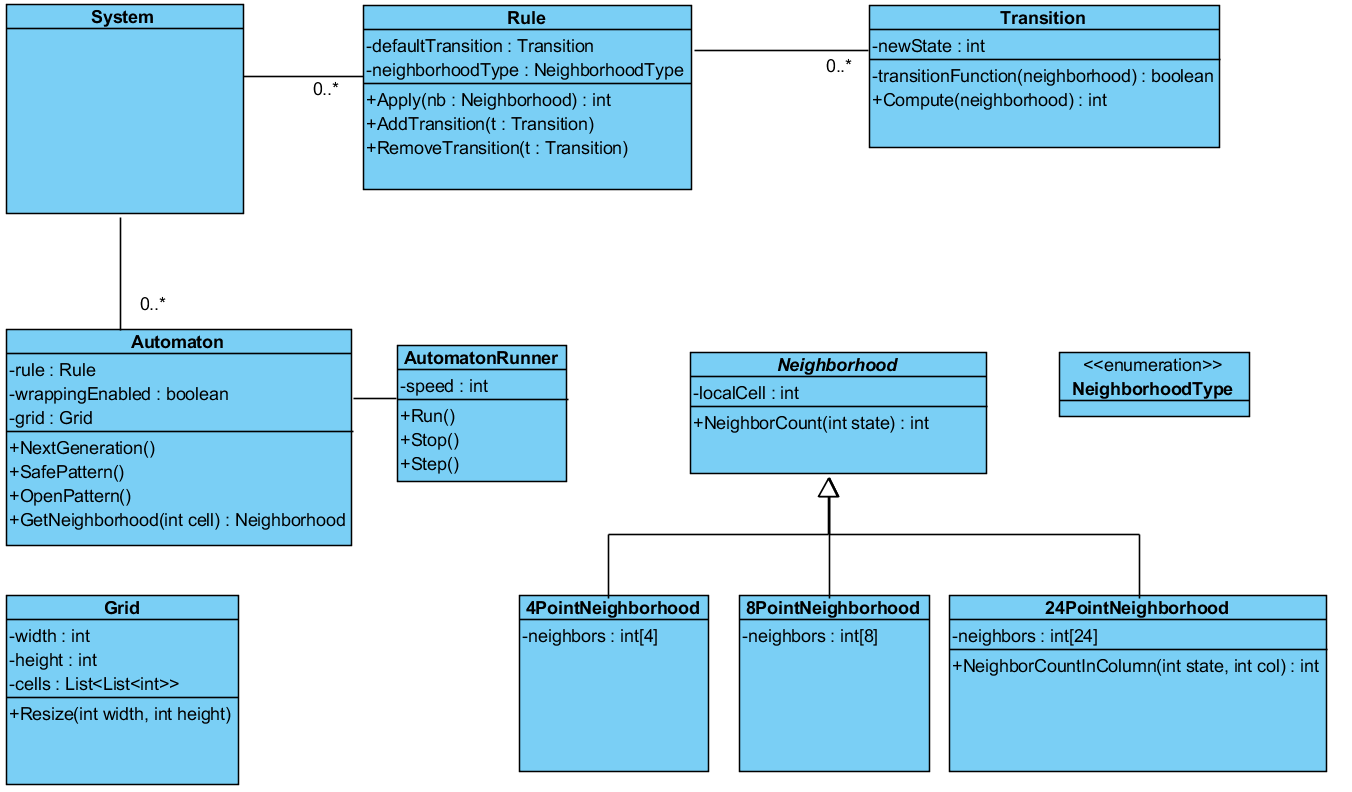
\includegraphics[width=180mm, height=100mm]{images/class_d.png} \\
	
	\begin{itemize}
		\item {\bf System} - contains all existing automata and rules saved in memory.
		\item {\bf Rule} - a set of Transitions, used to compute new generation.
		\item {\bf Transition} - contains a new state and a pointer to a some function defining this transition.
		\item {\bf Automaton} - class encapsulating cellular automaton.
		\item {\bf Grid} - data structure representing the cellular automaton in 2D
		\item {\bf Neighborhood} - Defines different neighborhoods.
		\item {\bf AutomatonRunner} - responsible to run Automaton.
	\end{itemize}
	
	\subsection{Use cases}

	\subsubsection{Automaton use cases}
		\hspace{-60pt}
		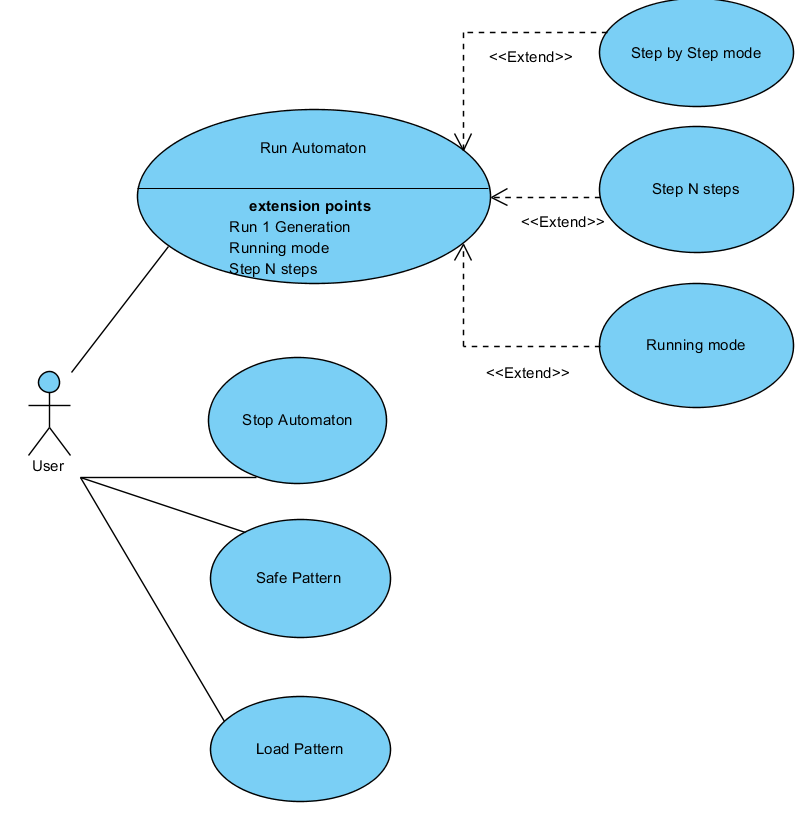
\includegraphics[width=100mm, height=100mm]{images/use_automaton_d.png} \\	
	
	\subsubsection{Editor use cases}
		\hspace{-60pt}
		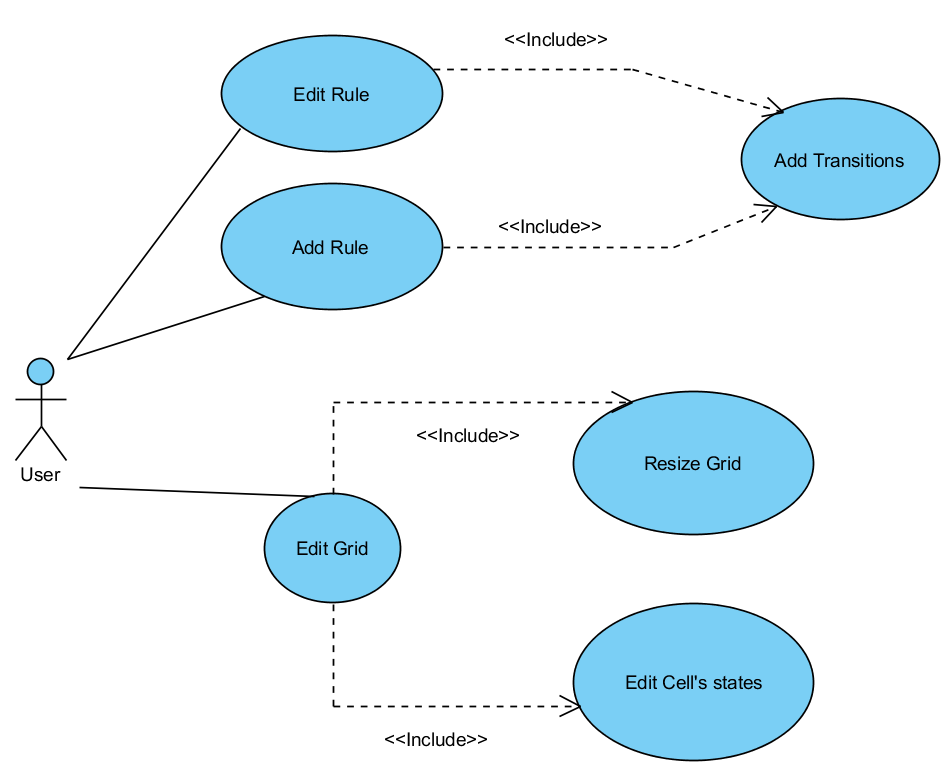
\includegraphics[width=100mm, height=100mm]{images/use_edit_d.png} \\	
				
				
	\subsection{State diagrams}


	\subsubsection{Editor}


		\hspace{-120pt}
		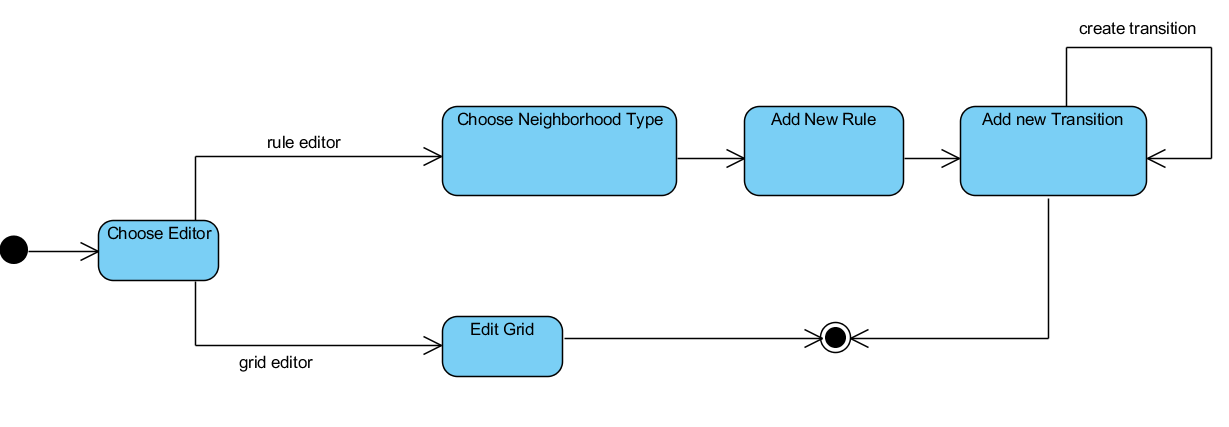
\includegraphics[width=200mm, height=100mm]{images/state_edit_d.png}
		
	\subsubsection{Automaton}
		\hspace{-90pt}
		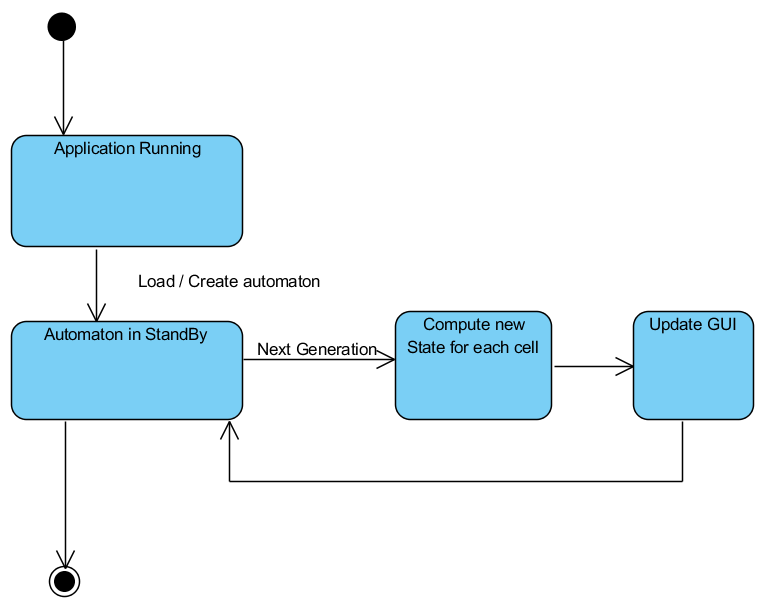
\includegraphics[width=150mm, height=100mm]{images/state_automaton_d.png} \\	
		
	
\end{document}
